%"runningheads" enables:
%  - page number on page 2 onwards
%  - title/authors on even/odd pages
%This is good for other readers to enable proper archiving among other papers and pointing to content.

%Even though `american`, `english` and `USenglish` are synonyms for babel package (according to https://tex.stackexchange.com/questions/12775/babel-english-american-usenglish), the llncs document class is prepared to avoid the overriding of certain names (such as "Abstract." -> "Abstract" or "Fig." -> "Figure") when using `english`, but not when using the other 2.
\documentclass[runningheads,a4paper]{llncs}
\usepackage[english]{babel}
\usepackage[utf8]{inputenc}

%better font, similar to the default springer font
%cfr-lm is preferred over lmodern. Reasoning at http://tex.stackexchange.com/a/247543/9075
\usepackage[%
rm={oldstyle=false,proportional=true},%
sf={oldstyle=false,proportional=true},%
tt={oldstyle=false,proportional=true,variable=true},%
qt=false%
]{cfr-lm}
%
%if more space is needed, exchange cfr-lm by mathptmx
%\usepackage{mathptmx}

\usepackage{graphicx}

%extended enumerate, such as \begin{compactenum}
\usepackage{paralist}

%put figures inside a text
%\usepackage{picins}
%use
%\piccaptioninside
%\piccaption{...}
%\parpic[r]{\includegraphics ...}
%Text...

%Sorts the citations in the brackets
%\usepackage{cite}

\usepackage[T1]{fontenc}

%for demonstration purposes only
\usepackage[math]{blindtext}

%for easy quotations: \enquote{text}
\usepackage{csquotes}

%enable margin kerning
\usepackage{microtype}

%tweak \url{...}
\usepackage{url}
%nicer // - solution by http://tex.stackexchange.com/a/98470/9075
\makeatletter
\def\Url@twoslashes{\mathchar`\/\@ifnextchar/{\kern-.2em}{}}
\g@addto@macro\UrlSpecials{\do\/{\Url@twoslashes}}
\makeatother
\urlstyle{same}
%improve wrapping of URLs - hint by http://tex.stackexchange.com/a/10419/9075
\makeatletter
\g@addto@macro{\UrlBreaks}{\UrlOrds}
\makeatother

%diagonal lines in a table - http://tex.stackexchange.com/questions/17745/diagonal-lines-in-table-cell
%slashbox is not available in texlive (due to licensing) and also gives bad results. This, we use diagbox
%\usepackage{diagbox}

%required for pdfcomment later
\usepackage{xcolor}

% new packages BEFORE hyperref
% See also http://tex.stackexchange.com/questions/1863/which-packages-should-be-loaded-after-hyperref-instead-of-before

%enable hyperref without colors and without bookmarks
\usepackage[
%pdfauthor={},
%pdfsubject={},
%pdftitle={},
%pdfkeywords={},
bookmarks=false,
breaklinks=true,
colorlinks=true,
linkcolor=black,
citecolor=black,
urlcolor=black,
%pdfstartpage=19,
pdfpagelayout=SinglePage,
pdfstartview=Fit
]{hyperref}
%enables correct jumping to figures when referencing
\usepackage[all]{hypcap}

%enable nice comments
\usepackage{pdfcomment}
\newcommand{\commentontext}[2]{\colorbox{yellow!60}{#1}\pdfcomment[color={0.234 0.867 0.211},hoffset=-6pt,voffset=10pt,opacity=0.5]{#2}}
\newcommand{\commentatside}[1]{\pdfcomment[color={0.045 0.278 0.643},icon=Note]{#1}}

%compatibality with TODO package
\newcommand{\todo}[1]{\commentatside{#1}}

%enable \cref{...} and \Cref{...} instead of \ref: Type of reference included in the link
\usepackage[capitalise,nameinlink]{cleveref}
%Nice formats for \cref
\crefname{section}{Sect.}{Sect.}
\Crefname{section}{Section}{Sections}

\usepackage{xspace}
%\newcommand{\eg}{e.\,g.\xspace}
%\newcommand{\ie}{i.\,e.\xspace}
\newcommand{\eg}{e.\,g.,\ }
\newcommand{\ie}{i.\,e.,\ }

%introduce \powerset - hint by http://matheplanet.com/matheplanet/nuke/html/viewtopic.php?topic=136492&post_id=997377
\DeclareFontFamily{U}{MnSymbolC}{}
\DeclareSymbolFont{MnSyC}{U}{MnSymbolC}{m}{n}
\DeclareFontShape{U}{MnSymbolC}{m}{n}{
    <-6>  MnSymbolC5
   <6-7>  MnSymbolC6
   <7-8>  MnSymbolC7
   <8-9>  MnSymbolC8
   <9-10> MnSymbolC9
  <10-12> MnSymbolC10
  <12->   MnSymbolC12%
}{}
\DeclareMathSymbol{\powerset}{\mathord}{MnSyC}{180}

% correct bad hyphenation here
\hyphenation{op-tical net-works semi-conduc-tor}

\usepackage[normalem]{ulem}

% \def\OP#1{{\color{red}OP: \it #1}}
% \def\ODdel#1{\bgroup\markoverwith{\textcolor{red}{\rule[0.5ex]{2pt}{1pt}}}\ULon{#1}}
\def\OP#1{#1}  % do nothing - disable the comments in whole documment

\definecolor{darkgreen}{rgb}{0.0, 0.5, 0.0}
\def\OD#1{{\color{darkgreen}OD: \it #1}}
\def\ODdel#1{\bgroup\markoverwith{\textcolor{darkgreen}{\rule[0.5ex]{2pt}{1pt}}}\ULon{#1}}
%\def\OD#1{\relax} % make my comments vanish
%\def\ODdel#1{#1} % make my comments vanish

\begin{document}

%Works on MiKTeX only
%hint by http://goemonx.blogspot.de/2012/01/pdflatex-ligaturen-und-copynpaste.html
%also http://tex.stackexchange.com/questions/4397/make-ligatures-in-linux-libertine-copyable-and-searchable
%This allows a copy'n'paste of the text from the paper
\input glyphtounicode.tex
\pdfgentounicode=1

\title{Dataset of operator-client dialogues aligned with knowledge-base queries}

\author{Ondřej Plátek \and Filip Jurčíček}
\institute{Charles University in Prague, Faculty of Mathematics and Physics \\
Institute of Formal and Applied Linguistics \\
Malostranské náměstí 25, 11800 Praha 1, Czech Republic \\
\email{\{oplatek,jurcicek\}@ufal.mff.cuni.cz}}

\iftrue % FIXME uncomment for final submission
\author{Firstname Lastname \and Firstname Lastname }
\institute{
Insitute\\
\email{anonym@anonymous}
}
\fi
			
\maketitle
% \OP{Fill missing values about the dataset collected so far} \\
% \OP{grammar check} \\

\begin{abstract}
    This paper presents a novel dataset for training end-to-end task oriented conversational agents.
    The dataset contains task oriented conversations between an operator – a task expert, and a client who is seeking information about the task, along with records of database API calls performed by the operator, which capture the distilled meaning of the user query.
    We expect that thanks to this easy-to-get supervision of database calls one would require significantly less training data for training end-to-end dialogue agents.
 	The dataset is collected using crowdsourcing on well known restaurant domain.
    The quality of the data is enforced by mutual control among contributors and manually verified on random sub-sample.
    The dataset is available for download under the Creative Commons 4.0 BY-SA license.
\end{abstract}

\vspace{-1.00em}
\keywords{task-oriented dialogue, end-to-end, dataset}
\vspace{-1.00em}

%%%%%%%%%%%%%%%%%%%%%%%%%%%%%%%%%%%%%%%%%%%%%%%%%%%%%%%%%%%%%%%%%%%%%%%%%%%%%%%
\section{Introduction}\label{sec:intro}
\vspace{-0.50em}
We present a new dataset of human-human task-oriented conversations in the restaurant info domain for supervised training of autonomous systems. 
Currently, the dataset contains only \OP{62} dialogues because we are still collecting more data, but we estimate that until camera ready deadline we will have more than seven hundreds dialogues. 
We aim at representing the conversation in such way that it is easy to train a system to replace an operator who provides information about the restaurants to clients.
In contrast to previously released datasets, our dataset contains easy to collect high-quality transcriptions of the client and operator actions during conversations.
We introduce a~very little overhead by collecting database calls in addition to the transcription of the conversation. 
In fact, we mimic very closely a~real situation in call centers where operators searches for answers through database user interface. 
On the other hand, just logging the calls to the task database provide us with information of the similar quality as it is contained in manually annotated dialogue state, just not annotated incrementally after each turn.
Tracking the database calls in task oriented systems together with conversation transcription should not introduce much overhead during data collection, but should presumably boost end-to-end conversational agent as much as annotated dialogue state when training with such data.

Current Spoken Dialogue Systems (SDS) are either handcrafted and use no training data~\cite{duvsek2014alex,raux2005let}, but require non-trivial amount of expert work, or are gradually improved from initial policy through live user interaction~\cite{young2010hidden,gasic2011line}, and lately are trained using supervised learning typically in end-to-end manner~\cite{wen2016network,williams2016end}.\footnote{The~work of \cite{williams2016end} also fine tuned the conversation with reinforcement learning after the supervised-learning stage.}
The reinforcement learning need just collect enough live user conversation containing only explicit feedback, but because the feedback signal is typically simple, noisy and delayed one require thousands of live conversations to improve rather simple policy.\cite{gasic2011line}
The supervised-learning methods greatly reduced the number of conversation needed for training reasonable policy to few hundreds\cite{wen2016network}, but require annotation for all components used the dialogue which so far included at least a dialogue state\cite{wen2016network,young2010hidden}.
Since the dialogue state is simplification of dialogue history and has no broadly-accepted form, it is very expensive to collect such annotated data because the dialogue state typically differs among domains and its structure is hard to explain to annotators.
In this paper, we focus on collecting supervised training set with rich enough annotation so the supervised models similar to~\cite{wen2016network} can be trained with few hundreds of dialogues, but the annotation of dialogues are much easier to collect.

We believe that our dataset dataset can be used for first experiments of training end-to-end systems using supervised learning without annotated dialogue state.
The domain of the dataset is well established thanks to dialogue state tracking (DST) challenges~\cite{williams2013dstc1,henderson2014dstc2,henderson2014dstc3}. 
The DST challenges proved that the domain is of reasonable complexity.
In addition, the challenges showed that the DST task is solvable by architectures which may be extended to end-to-end conversational agents~\cite{platek2016recurrent,vodolan2015hybrid,henderson2014word}.
Note that we collected human-to-human dialogues on Cambridge restaurant domains, but our data-collection method is domain independent.

The paper is structured as follows: Section~\ref{sec:repre} motivates the annotations and format of our dataset.
In Section~\ref{sec:collection} we introduce our collection process using crowdsourcing.
Section~\ref{sec:props} presents the dataset properties and we list the related work in Section~\ref{sec:related}.
We conclude the paper and suggest future work in~Section~\ref{sec:conc}.

% \section{End-to-end training of dialogue systems}
% \label{sec:training}

\section{Supervised feedback for task-oriented dialogue} \label{sec:repre}
\vspace{-0.50em}
We present a dataset for training a task-oriented conversational agent in well defined domain.
We assume that the agent has a task database\footnote{In the Cambridge restaurant domain the database is a simple table containing information about restaurants.} at hand and plays role of {\it operator}.
The other interlocutor in the conversation is a~human {\it client}.
{\it Clients} seek information stored in the database and use the system, which replaced a~human operator, to obtain desired information.

We focus on data collection for text-to-text task-oriented dialogue systems.
Traditionally, one would train the pipeline of components of task-oriented dialogue systems, i.e.\ automatic speech recognition (ASR), language understanding (LU) unit, dialogue tracker (DT), dialogue manager (DM), natural language generator (NLG) for text-to-text conversational agents and text-to-speech (TTS) module~\cite{duvsek2014alex}.
However, typically only the text-to-text pipeline of LU, DT, DM and NLG is trained using just the domain-related text-to-text data~\cite{gasic2011line,jurvcivcek2014factored,duvsek2016sequence}.
The ASR~\cite{platek2014free} and the TTS~\cite{taylor2009text} modules are typically trained using larger datasets.
Our datasets contains data for training an~end-to-end system solving task of LU, DT, DM and NLG pipeline of traditional architecture.

% Me to nesedi jako related work - related work je o sbirani dat
% Tohle me prijde zduvodneni, ze takovy (maly, supervised) dataset dava smysl
% Zatim nechavam zde: \OD{následující dva odstavce zní dost jako “related work”... možná bych to tam částečně popřesouval? a tady nechal jen ten statement, že stačí málo trénovacích dat?}
It was shown that few hundreds of annotated domain specific conversations is needed for training relatively well performing LU~\cite{jurvcivcek2014factored} as well as Dialogue State Tracking~\cite{young2010hidden} components.
The work of~\cite{duvsek2016sequence} and~\cite{mairesse2010phrase} showed that only several hundreds of turns with appropriate annotation is needed for training usable NLG unit on simple domains.
Even the crucial task of action selection with reward provided only at the end of dialogue can be trained using POMDP dialogue manager and few thousands conversations~\cite{gasic2011line}.

We believe that end-to-end systems even with latent variables can be trained using few hundreds conversation if additional supervision in the form of simple annotation is used for narrow goal-oriented domains such as~\cite{wen2016network} domain or Cambridge restaurant domain~\cite{henderson2014dstc2}.
A~recent work of~\cite{wen2016network} showed that only 680 conversation annotated with just at dialogue state level is needed for training the whole end-to-end system performing the task of summarizing the dialogue history and reply planning and generation on a very simple domain.

We note that further annotation of dialogue conversation may help to train the models faster, but simply collecting more data is typically more beneficial.
As a consequence, we see works~\cite{wen2016network,bordes2016learning,williams2016end} as important step forward not to rely on rich annotations for training dialogue agents.
We believe that annotating a dialogue state according to expert-handcrafted ontology is both an~artificial and a~very labor-intensive data collection task, so our work aim at collecting conversation with lighter but more easier to get annotations.
We suggest to record conversation between human operator and human clients through crowdsourcing and by this means collect cheap high quality training data.
Similar recording setup is known from call centers where the operator is provided with interface to the database so it quickly finds relevant information and plays the role of domain expert.
We suggest to collect the operator's database calls with its arguments instead of dialogue state annotation after each turn.

The calls to the database completely represents the client intention which is the purpose of the dialogue state.
On the other, the database calls are not present in every turn and thus by logging only the calls one loses a possibility to track partially filled client intention.
We argue that in high quality human-human conversation there is a minimum turns which are related to the domain and do not contain calls to the database as demonstrated in~Section~\ref{sec:props}.
It's worth noting that logging operator's database calls in operator-client dialogues is already well established practice in call centers, a~convenient field for commercial application of dialogue systems.

\section{Dataset Collection Process} \label{sec:collection}
\vspace{-0.50em}
Our data collection processed aimed at collecting natural conversation in the well defined domain.
We decided to collect new dataset int the~well studied Cambridge restaurant domain since the previous datasets~\cite{williams2013dstc1,henderson2014dstc2,henderson2014dstc3} in that domain demonstrated that a meaningful and of a reasonable length conversation can be held in the domain.
Also it was proven that the domain is on one hand difficult enough that even the state-of-the art systems does not reach human-level performance in the role of the operator~\cite{henderson2014dstc2} and on the other hand numerous systems~\cite{young2010hidden,gasic2011line,wen2016network} demonstrated that are able to provide information to the clients reasonable well.

We define our domain by choosing a database from Dialogue State Tracking Challenge 2 (DSTC2)~\cite{henderson2014dstc2}.
We use the database for steering the dialogue of the two human interlocutors a~{\it client} and an~{\it operator}.
We use the CrowdFlower (CF) crowdsourcing platform for collecting the conversations.

We first describe the database which defines our domain in~Section~\ref{sec:db}.
Then we describe how the hired workers used our interface for playing either client or operator roles in~Sections~\ref{sec:client} and~\ref{sec:operator}.
Finally, in~Section~\ref{sec:async} we describe how we collected conversations one response at a time without connecting the interlocutors in real-time. 

\vspace{-1.00em}
\subsection{Domain database}
\label{sec:db}

We used exactly the same database as provided for the DSTC2 challenge~\cite{henderson2014dstc2}.
The database contains information about 107 restaurants and their properties stored in the columns.
We include in brackets the number of different values for each column:
\vspace{-0.50em}
\begin{itemize}  % tabulku misto tohohle?
    \item name (107),
    \item price range (4),
    \item area (7),
    \item food (25),
    \item address (101),
    \item phone (97),
    \item postcode (62).
\end{itemize}
\vspace{-0.50em}

The address or the phone are unique for each restaurant but are sometimes missing, but the name of the restaurant is always known. 
There are typically multiple restaurant with the same postcode, price range, area, or food type property and these properties might be unknown for a restaurant.

We use the database to generate client goals for CF users (see Figure~\ref{fig:client}), and CF users playing role of the operator can directly access and search the database (see Figure~\ref{fig:operator}).

\vspace{-1.00em}
\subsection{Client interface}
\label{sec:client}

The client is given a goal to request provided information from the operator.
He may choose not to seek the goal immediately but submit more appropriate response such as greeting first.
The goals are displayed to the CF worker in the client role gradually turn-by-turn and the goals may contradict each other.
For example, the client may at first want a Chinese food, but later it changes her mind and wants to find restaurant serving British food.

Before submitting a reply the client is instructed to read the dialogue history and marked the goals which were presented to the operator as demonstrated in Figure~\ref{fig:client}.
By marking which goals have been already presented to the operator we force the CF workers to pay attention to the dialogue history before submitting their reply.
In Section~\ref{sec:async} we describe how we combine the workers replies to conversations.

\begin{figure}
\vspace{-1.00em}
\begin{center}
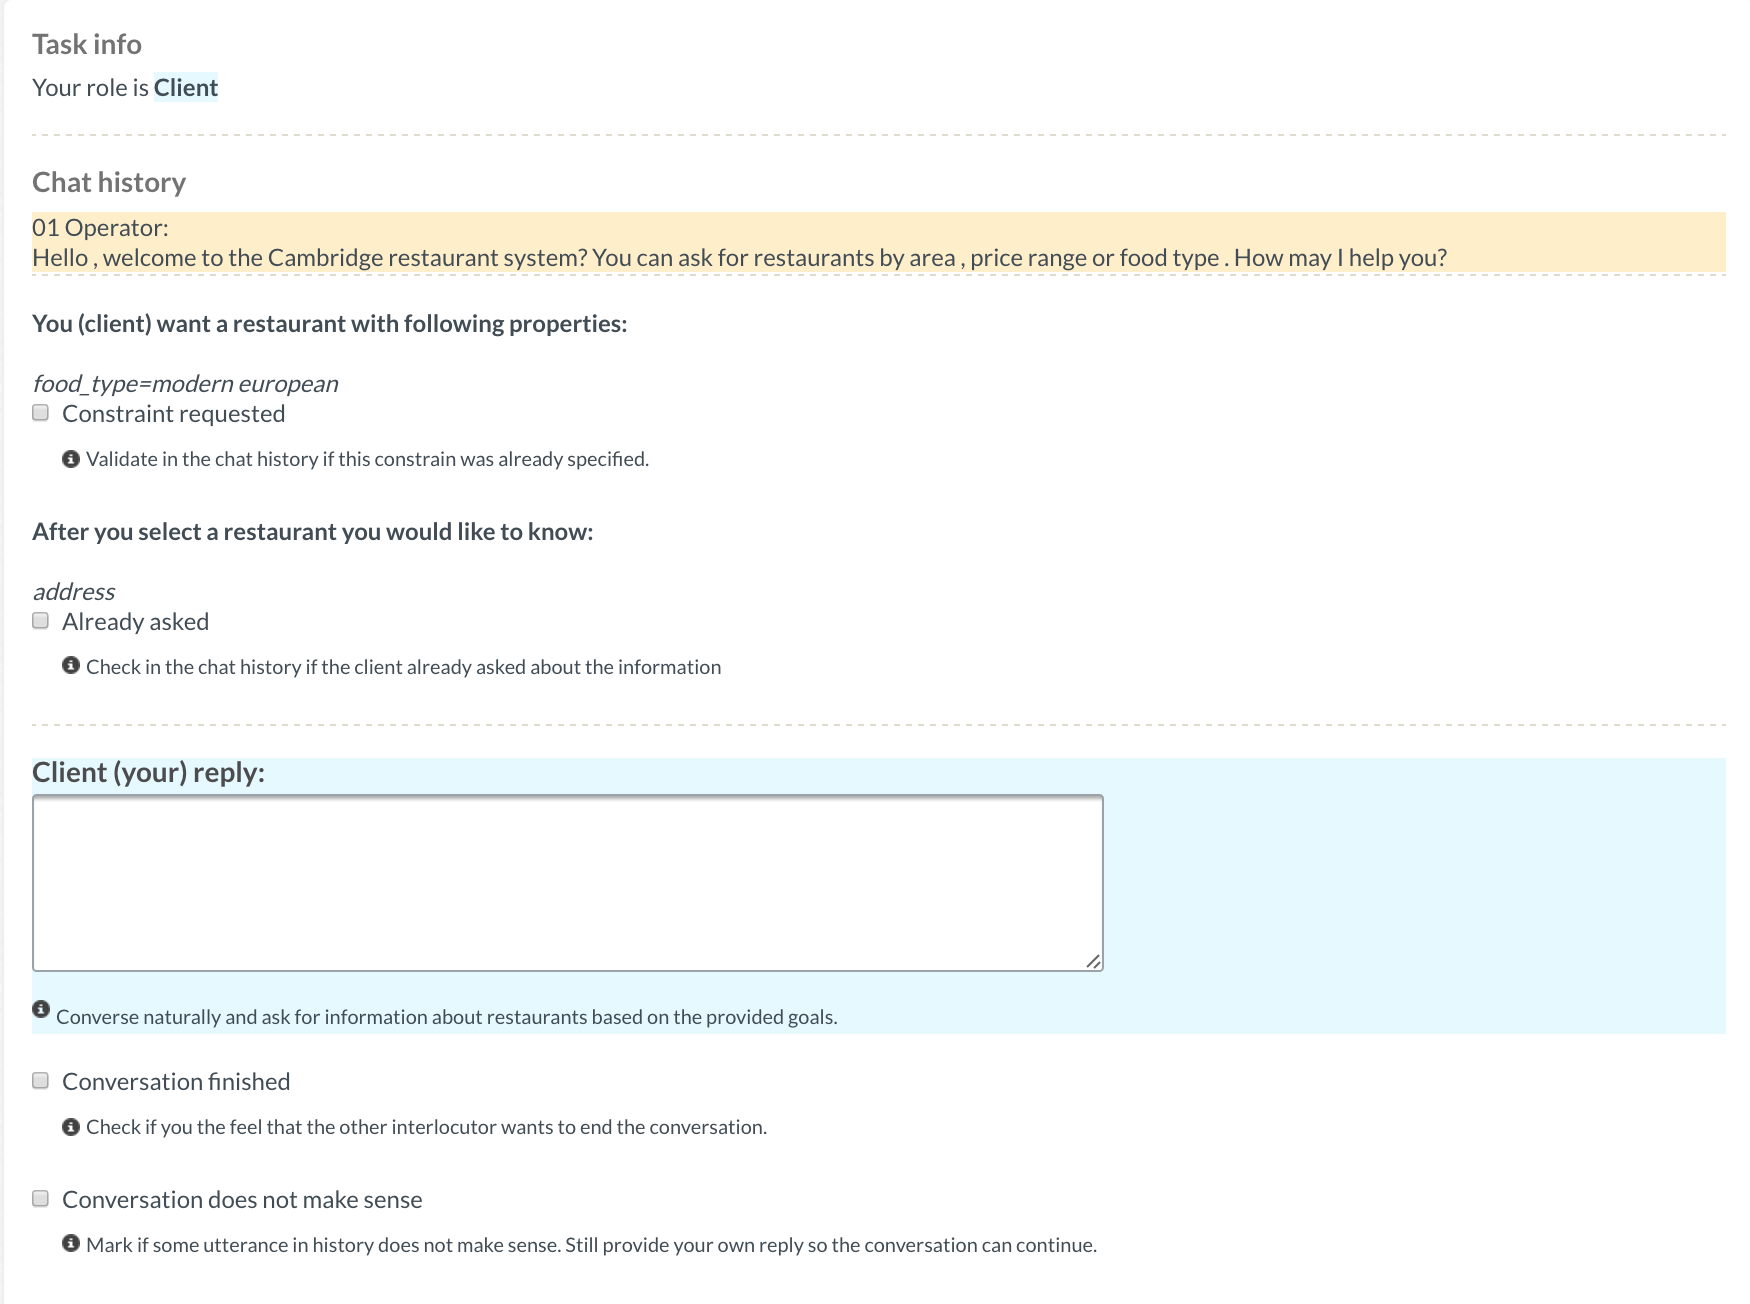
\includegraphics[height=30em]{gui-annotators-client}
\caption{Client annotation interface}
\end{center}
\vspace{-1.00em}
\label{fig:client}
\end{figure}
\vspace{-1.00em}

\vspace{-1.00em}
\subsection{Operator interface}
\label{sec:operator}
The operator is asked to politely reply the clients needs according the information stored in the database.
In order to provide the information to clients the operator uses the DB interface depicted in~Figure~\ref{fig:operator}.
Her or she filters the restaurants using a full text search on the database.
The content of the database is intentional hidden if no filter is specified so the filter has to be used.
The CF workers are also instructed also explicitly mark the rows of the restaurants about which provide the information in their answer.
Similarly to the client role, an operator does not have to reply to all requested information at once.
It is up to worker which information is provided first.

The full text search, our interface to the database, is implemented in Javascript as a simple substring matching over values in the database.
Multiple constrains can be expressed by two substrings separated by a comma.
We used such a simple interface because it is easy to generate the candidate results given the query and the database.
The CF workers were instructed to mark a candidate row from the results about which they inform in their reply.

\begin{figure}
\vspace{-1.00em}
\begin{center}
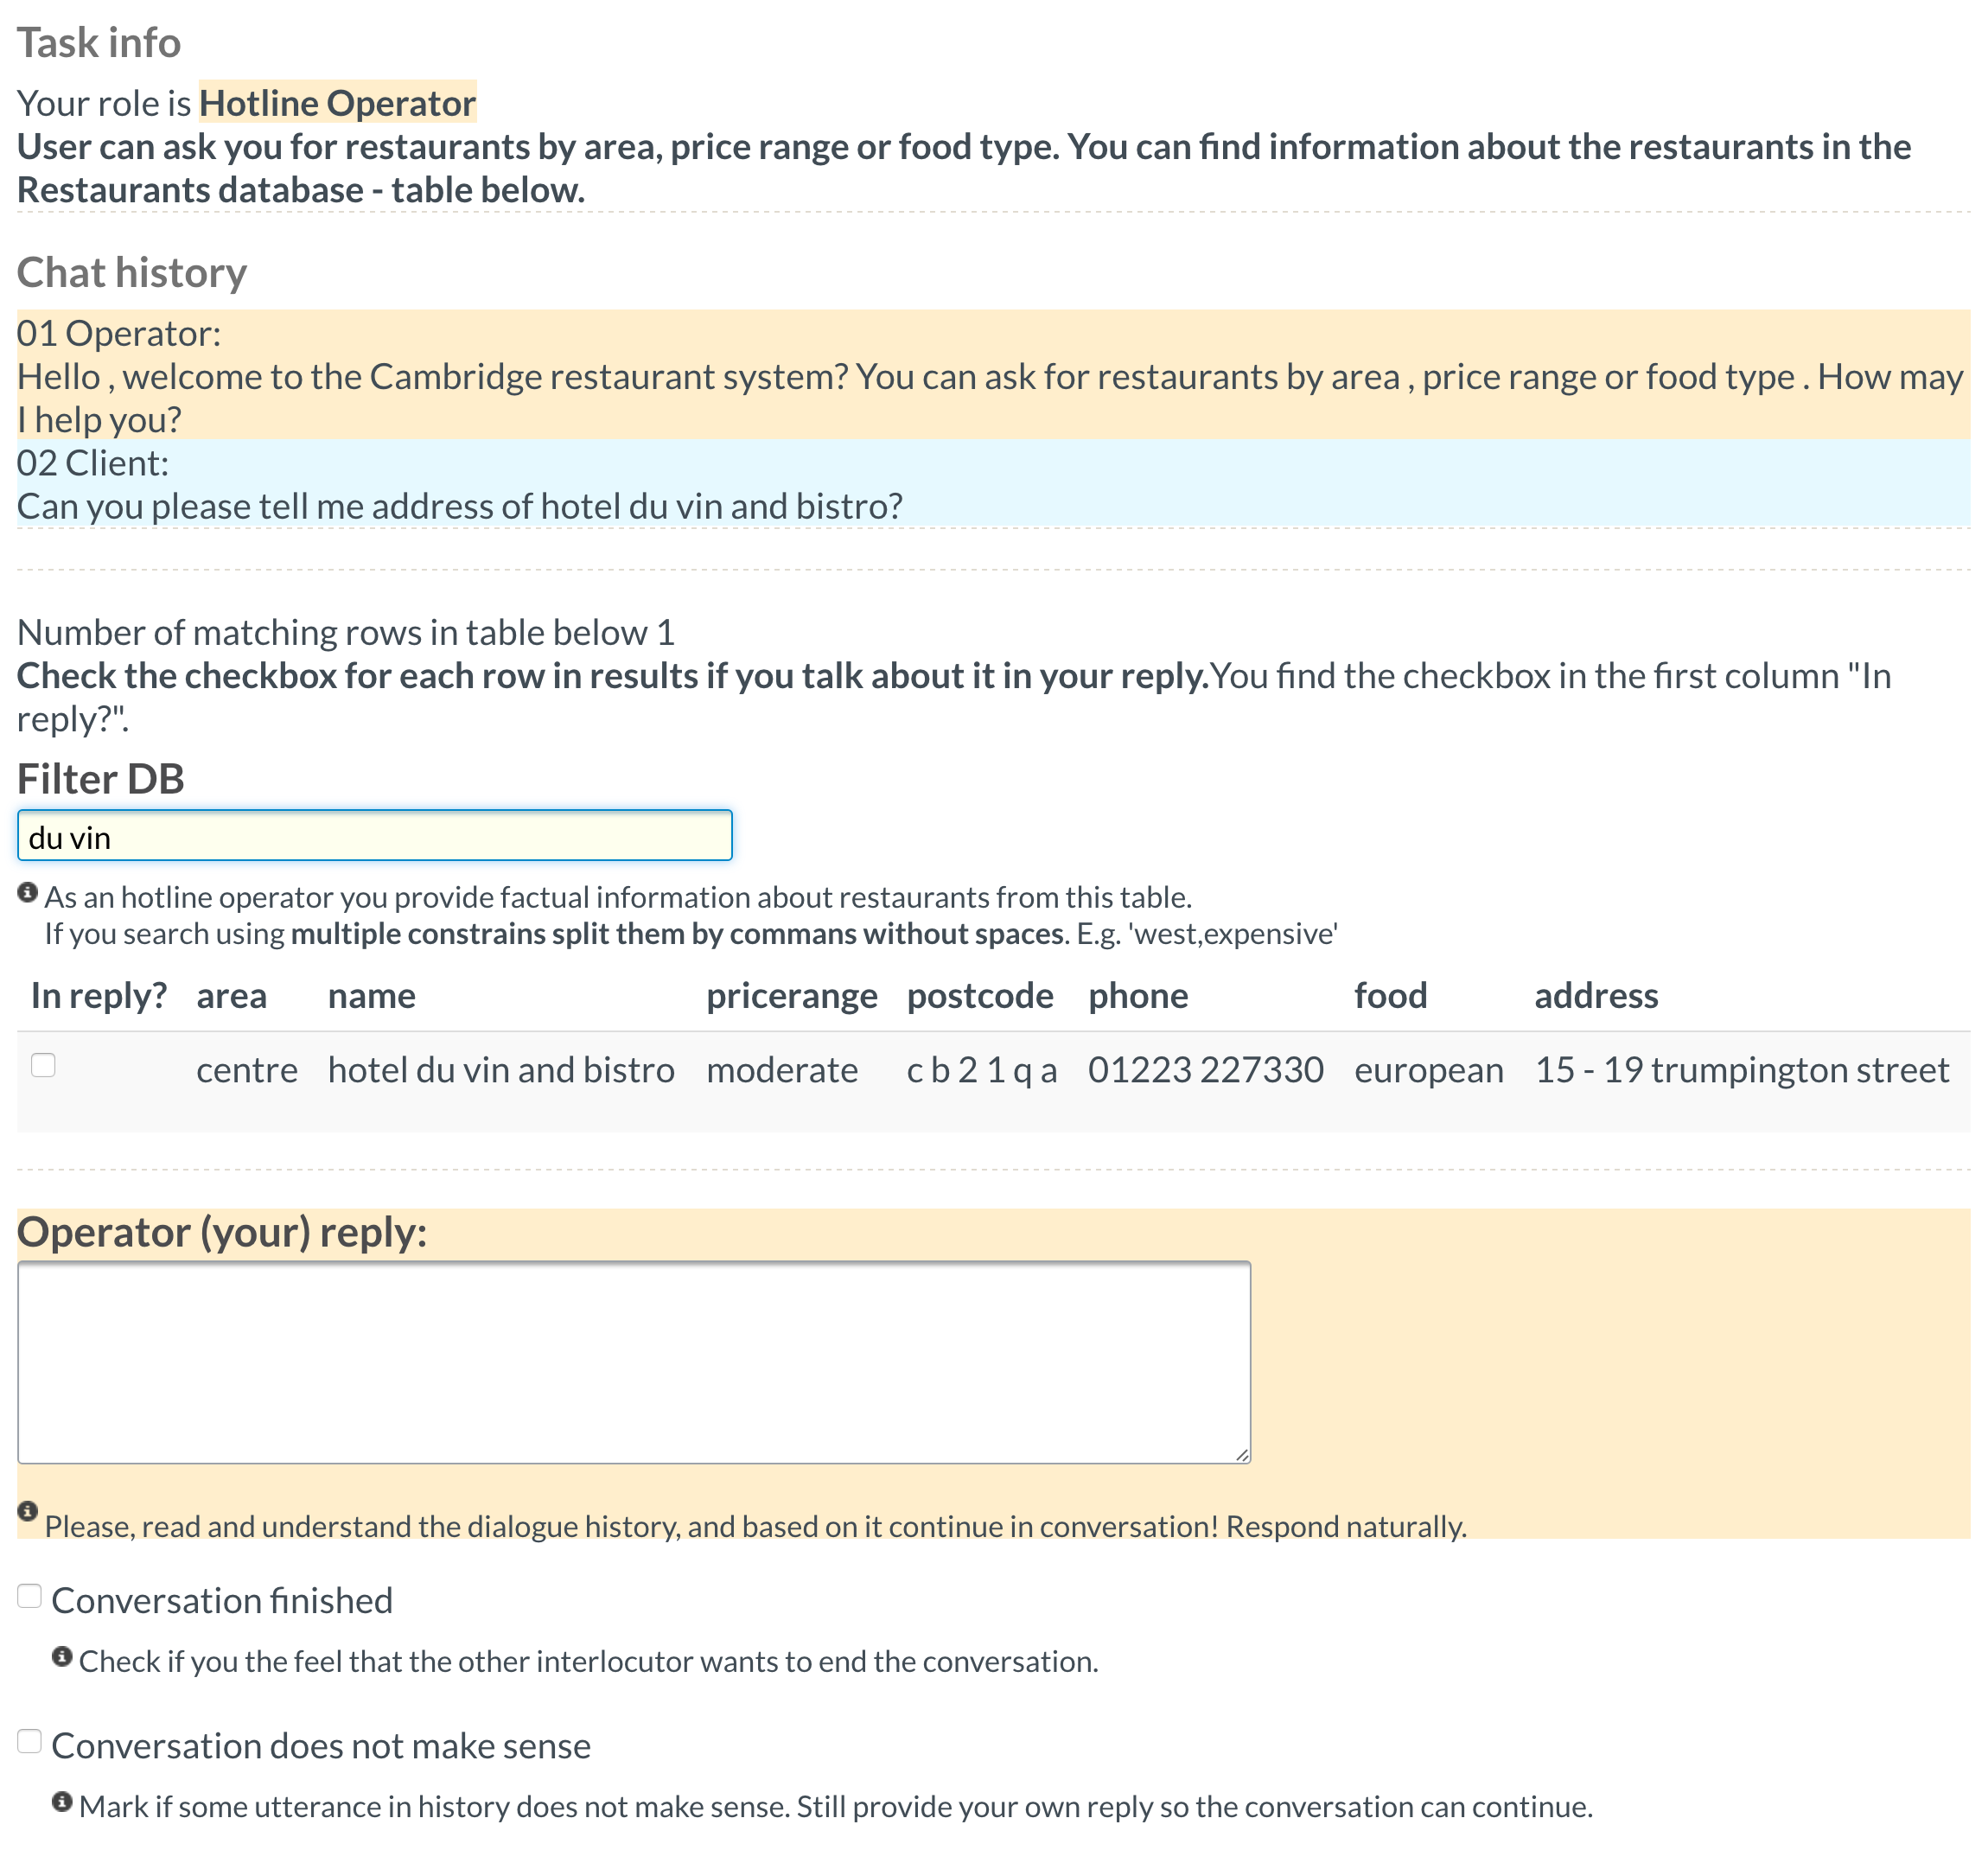
\includegraphics[height=35em]{gui-annotators-system}
\caption{Operator annotation interface}
\end{center}
\vspace{-1.00em}
\label{fig:operator}
\end{figure}
\vspace{-1.00em}

\vspace{-1.00em}
\subsection{Asynchronous collection without real-time responses}
\label{sec:async}
We design the crowdsourcing jobs so the CF contributors are able to work independently to each other.
The roles of client and operator take turns as sets of partial conversations are submitted for collecting a single new response.
As a consequence, multiple contributors participate in submitting responses for single conversation for both roles.

Each utterance in conversation may be submitted by different contributor, so contributors need to read carefully the dialogue history to understand the conversation before submitting their response.
The workers are able to mark dialogues which does not make sense and thus they self-assess quality of the conversations.
The contributors mark the conversations as finished if they have no more goals to fulfill and all the goodbyes were said.

We bootstrap the conversation either with an operators introduction "{\it Hello , welcome to the Cambridge restaurant system...}" or we bootstrap the conversation with a~full turn where we add clients greeting e.g. {\it "Hi"} to aforementioned operators utterance.
If we initialize the dialogue with a~full turn the first contributor plays role of the system if we bootstrap the conversation only with~the operators greeting, the contributors plays the client's role.

In single job submission we let the workers append to each dialogue a~single response.
Note also that the conversations are typically rather short so full dialogues are collected after few rounds of submissions.
The workers are paid for every submitted response the same amount independently if they play client or operator role and they typically contribute to multiple conversation during one job submission.
The contributors are assigned roles randomly.

To avoid poor language level of English we restricted the CF worker to English-speaking countries.
We further perform heuristically check for too trivial answers and we added ability to the CF workers to rate each others submission.
It help us filter low quality conversations, but more importantly it motivated workers not to cheat.

\section{Dataset Properties} \label{sec:props}
\vspace{-0.50em}
We just started to collect our dataset and so far we collected only 60 conversations.
The average length of a conversation is \OP{3.8} turns, meaning that the contributors and in both roles reply three times before the conversation is finished\footnote{First system reply is automatically generated and for some conversation even the first client reply is also initialized as described in Section~\ref{sec:async}}.
During an average conversation \OP{2.4} tasks are requested and \OP{1.9} answered.
% Typically in \OP{65} \% case the conversation is ended by the client.
% As we mention the conversation are short, taking only from \OP{four to six turns} including first turn with greetings.
% \begin{table}
% \begin{center}
% \begin{tabular}{lrr}
% \hline
% Set   & \# Dialogues & \# Turns \\
% \hline
% % Joint  &  todo &  todo \\
% % /a/SSD/oplatek/e2end/log/2016-06-08-17-31-38.400-dstc-INDEP_labels-d0.7-w100-e100/
% % /a/SSD/oplatek/e2end/log/TEST-ORIGINAL-2016-06-08-17-31-38.400dstc-INDEP_labels-d0.7-w100-e100-reward-0.9080-step-0036224
% Train  &   ? & ? \\
% Dev &   ? & ? \\
% Test &   ? & ? \\
% \hline
% \end{tabular}
% \caption{Accuracy on development and test set}
% \vspace{-2em}
% \end{center}
% \label{tab:props}
% \end{table}
During the data collection process we discarded over \OP{20} \% of replies because the utterances were of low quality.
Note that we discard only the low quality utterance, the prefix of the conversation is submitted for finishing the conversation in next rounds of jobs.
Once we will collect enough conversation we intend to split them into training, development and test set. % (see Table~\ref{tab:props}).


\section{Related Work} \label{sec:related}
\vspace{-0.50em}
Our work is closely related  to work of~\cite{williams2013dstc1,henderson2014dstc2,henderson2014dstc3} in the sense that the conversation are held in the same domain.
On the other hand, the collection process differs substantially because we do not use any artificial system and rather we focus on collecting high quality human conversations. In addition, in our work we do not collect complicated annotations on LU and DST level.

A~relevant work of~\cite{wen2016network} collected human-human dialogues in similar but more restricted domain than the Cambridge domain.
Their dataset is not yet published so we compare only with their statistics.
The dataset is of similar size and used very similar collection scheme where the Amazon Mechanical Turk workers submitted one reply at a time without being connected to each other in real-time.
On the other, hand they collected explicit dialogue state annotation which takes significant annotation effort.

Another line of research~\cite{vodolan2016data} used CF to collect human-human conversation for interactive-learning dataset.
However, the collected dialogues were later annotated by expert annotators which goes directly against our intentions to avoid any expensive annotations.

There is significant amount of work which used Wizard of Oz experiments~\cite{whittaker2002fish,walker1997evaluating,rieser2008learning} for studying linguistic properties of dialogues, evaluating proof of concept or even collecting bootstrap training data, but according our knowledge no other work than~\cite{wen2016network} have not used cheap crowdsourcing workers to collect a~full training dataset for supervised learning of dialogue management or end-to-end conversations.

\section{Conclusion and Future work} \label{sec:conc}
\vspace{-0.50em}
We present a new human-human dialogue dataset with annotation of user intention in form of their database calls.
We also introduced a novel data collection setting which resembles work of operators in call centers and introduce minimum overhead to crowdsourcing workers.
% TO mi prijde ze v call -centrech delaji stejne\OD{, apart from stating their replies in natural language (?)}
The collected dialogues are published under Creative Commons 4.0 BY-SA license on available to download at {\it anonymized}.  % lindat\footnote{todo where}.

We plan to increase the number of collected dialogues till the camera ready deadline to 700 or more.
We intend to use the dataset to train and evaluate an~end-to-end conversational model which uses only the database calls as additional supervision to the recorded responses. 

\vspace{-1.00em}
\subsubsection*{Acknowledgments}
We would like to thank Ondřej Dušek for useful comments.
This research was partly funded by the Ministry of Education, Youth and Sports of the Czech Republic under the grant agreement LK11221, core research funding, grant GAUK 1915/2015, and also partially supported by SVV project number 260 333. 
% We gratefully acknowledge the support of NVIDIA Corporation with the donation of the Tesla K40c GPU used for this research.
% Cloud computational resources were provided by the MetaCentrum under the program LM2010005 and the CERIT-SC under the program Center CERIT Scientific Cloud, part of the Operational Program Research and Development for Innovations, Reg.\ no. CZ.1.05/3.2.00/08.0144.

% ``something in quotes'' using plain tex or use \enquote{the enquote command}.
% cref Demonstration: Cref at beginning of sentence, cref in all other cases.
%
% \Cref{fig:simple} shows a simple fact, although \cref{fig:simple} could also show something else.
%
% \Cref{tab:simple} shows a simple fact, although \cref{tab:simple} could also show something else.
%
% \Cref{sec:intro} shows a simple fact, although \cref{sec:intro} could also show something else.
%
% Brackets work as designed:
% <test>
%
% The symbol for powerset is now correct: $\powerset$ and not a Weierstrass p ($\wp$).
%
% \begin{inparaenum}
% \item All these items...
% \item ...appear in one line
% \item This is enabled by the paralist package.
% \end{inparaenum}
% In the bibliography, use \texttt{\textbackslash textsuperscript} for ``st'', ``nd'', ...:
% E.g., \enquote{The 2\textsuperscript{nd} conference on examples}.
% When you use \href{http://www.jabref.org}{JabRef}, you can use the clean up command to achieve that.


% Winery~\cite{Winery} is graphical \commentontext{modeling}{modeling with one \enquote{l}, because of AE} tool.
%%%%%%%%%%%%%%%%%%%%%%%%%%%%%%%%%%%%%%%%%%%%%%%%%%%%%%%%%%%%%%%%%%%%%%%%%%%%%%%
\vspace{-1.00em}
\bibliographystyle{splncs03}
\bibliography{paper}
\vspace{-1.00em}

% All links were last followed on June 28, 2016.
%%%%%%%%%%%%%%%%%%%%%%%%%%%%%%%%%%%%%%%%%%%%%%%%%%%%%%%%%%%%%%%%%%%%%%%%%%%%%%%

\end{document}
